\documentclass{article}
% translate with >> pdflatex -shell-escape <file>

% This file is an extract of the PGFPLOTS manual, copyright by Christian Feuersaenger.
% 
% Feel free to use it as long as you cite the pgfplots manual properly.
%
% See
%   http://pgfplots.sourceforge.net/pgfplots.pdf
% for the complete manual.
%
% Any required input files (for <plot table> or <plot file> or the table package) can be downloaded
% at
% http://www.ctan.org/tex-archive/graphics/pgf/contrib/pgfplots/doc/latex/
% and
% http://www.ctan.org/tex-archive/graphics/pgf/contrib/pgfplots/doc/latex/plotdata/

\usepackage{pgfplots}
\pgfplotsset{compat=newest}

\pagestyle{empty}

\usepgfplotslibrary{polar}

\begin{document}
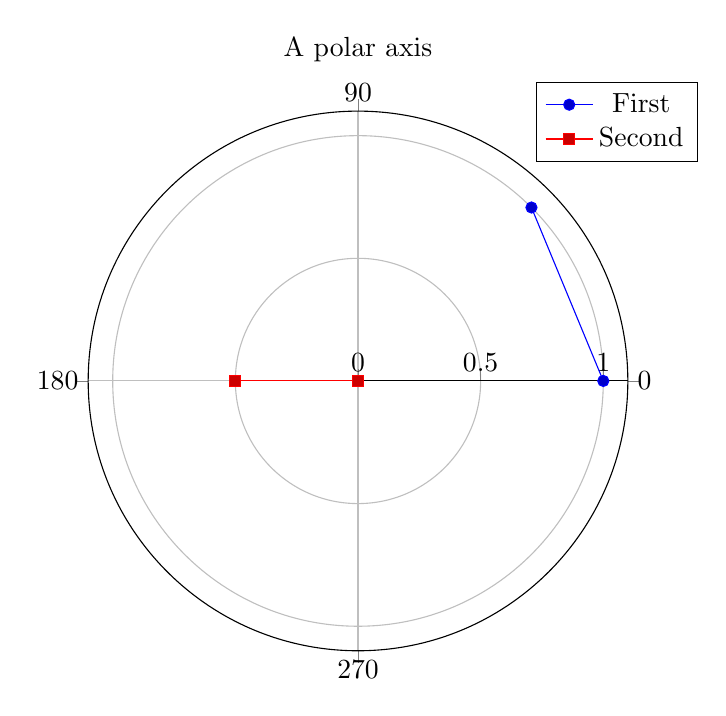
\begin{tikzpicture}
	\begin{polaraxis}[
		xtick={0,90,180,270},
		title=A polar axis]
	
	\addplot coordinates {(0,1) (45,1)};
	\addlegendentry{First}

	\addplot coordinates {(180,0.5) (0,0)};
	\addlegendentry{Second}
	\end{polaraxis}
\end{tikzpicture}
\end{document}
